\section{Madrid Metro}
\label{Madrid}

In this chapter will be developed a Zimulator model for the Madrid
Metro system.  The model is to be constructed using only public
sources of data, which are in cases of insufficiency supplemented with
synthetic data.  The resultant model is intended here solely to
function as an illustrative example of metro-system simulation.

All public data are extracted from Wikipedia.\footnote{Data are taken from \href{https://en.wikipedia.org/wiki/Madrid_Metro}{https://en.wikipedia.org/wiki/Madrid\_Metro} and associated pages.} All source addresses are included
as fields within the raw metro-system data files described below.

The level of detail of the model will be influenced by the form and
details of available data. Such a model is sufficient for illustrative
purposes; in the case of quantitative application to a metro system,
actual system data would be expected to produce a more realistic model.

\subsection{Metro system public data}

Available data describe the geometrical layout of the metro network,
in addition to the transit lines and connectivity. The extracted data
have been stored in three source files, the form of which is briefly
described here. This file format is nothing more than an intermediate
tool to create the zsyntax files which describe the system. It is a
simple ad-hoc format particular to the Madrid system, but may be
useful, with possible embellishments, in describing other metro
systems.

{\tt Line\_List.csv} -- This defines an index, code, name and source location for each of the 16 metro lines. 
An example row is: 
\begin{lstlisting}[mathescape]
  11,s,L11,Plaza Elíptica - La Fortuna,https://en.wikipedia.org/wiki/Line_11_(Madrid_Metro)
\end{lstlisting}
The field `s' indicates that the line is `straight' as opposed to a loop line, which would be indicated by `l'.

{\tt Station\_List.csv} -- This defines a three-letter code, name, latitude and longitude for each metro station. \\
An example row is:
\begin{lstlisting}[mathescape]
 SLS,San Lorenzo,40.4744713,-3.6395754,https://en.wikipedia.org/wiki/San_Lorenzo_(Madrid_Metro)
\end{lstlisting}  
The three-letter codes are generated for the purpose of the simulation, and are not official.

{\tt Itinerary\_List.csv} -- This file defines the paths taken by each line in the system, as a list of stations.
An example sequence of rows is:
\begin{lstlisting}[mathescape]
 5,1,ADO,0
 5,2,ECE,802.249
 5,3,LEA,1407.06
 . . .
 5,30,PAL,735.651
 5,31,CAT,579.064
 5,32,CDC,1226.36
\end{lstlisting}
This section of 32 rows in total indicates that transit line number 5 travels through
32 stops, from ADO to CDC.  The fourth field indicates the distance
in metres to the given stop from the previous stop.  In the present
case the distances have been estimated using the latitude and
longitude coordinates of each station, taking the geodesic distance
and multiplying arbitrarily by $1.1$.

These CSV files will be taken to be the raw system data; below in \secref{madseczsyn}
these data will be used to engineer the system in terms of Zimulator objects.

\subsection{Synthetic data}

The data mentioned in the previous section do not describe the system
comprehensively; while the infrastructure is thereby specified, the
supply and demand remain undetermined. These are generated synthetically.

\begin{figure}[ht]
  \centering
  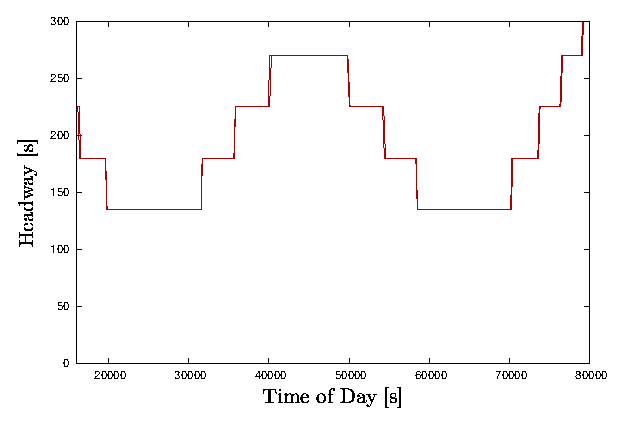
\includegraphics[angle=0,width=8cm]{70_figs/_headway_vs_ToD.eps}
  \caption{Headway depends on time of day.}
  \label{hwdep}
\end{figure}

\begin{figure}[ht]
  \centering
  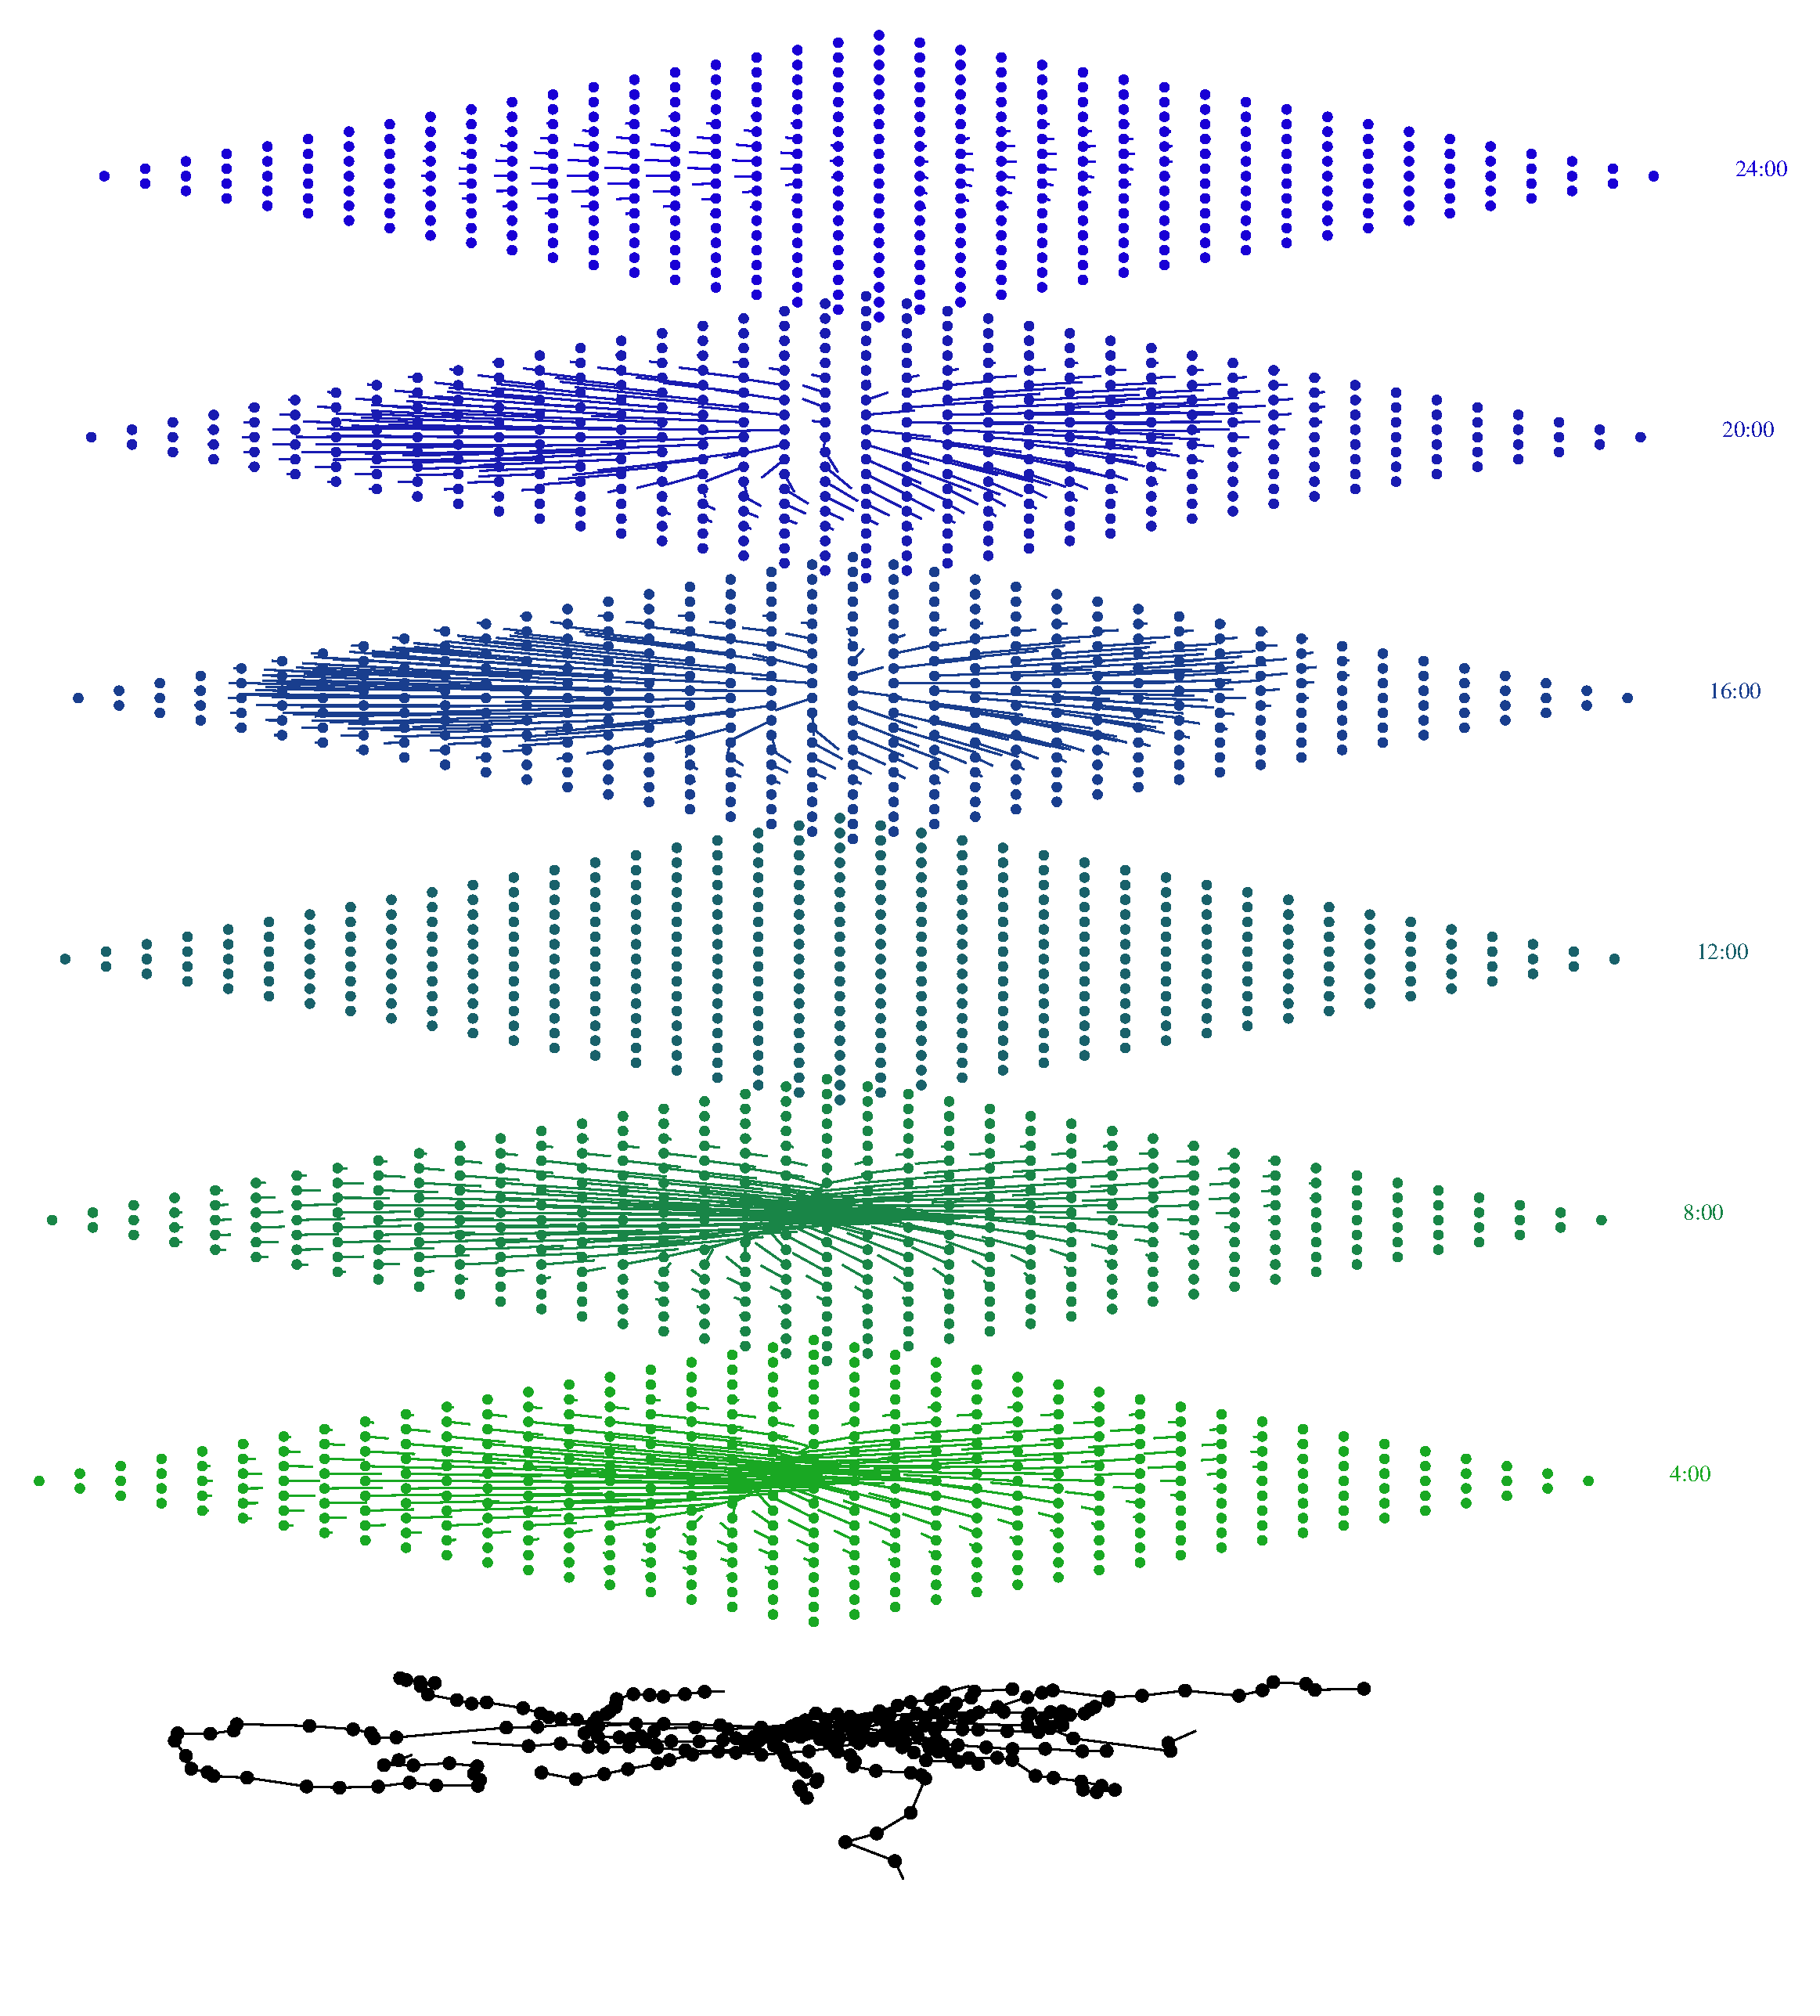
\includegraphics[angle=0,width=10cm]{70_figs/_SystemFlows.eps}
    \caption{Large-scale demand throughout the day.
      The figure shows the directional local net flow of passengers in a two-dimensional plane,
      at various times during the day. For spatial reference, a schematic of the
      transit lines is shown below the first slice. }        
  \label{demandinday}
\end{figure}
  
Trains are supplied on each of the lines at intervals, all day long
from approximately 04:30 to 25:00. The headway, shown in
\Figref{hwdep}, (time between subsequent train deployments) is modeled
very simply, to accommodate a higher train frequency during peak hours
of near 07:00 and 19:00.

The passenger demand is generated to represent the general flow within
an urban area; the flow of commuters is generally towards the city
centre during the morning peak period, and generally away from the
centre during the evening peak. There is no intention to model accurately the
flow in the actual city; the intention here is to provide an example day of
demand which is not entirely unrealistic. The sequence of passenger
flows throughout the day is indicated in \Figref{demandinday}.

\subsection{Station template}

The arrangement of each station in the metro system is that presented
earlier in \Figref{fig:STN}, with four gates associated with each
station. This is an arbitrary choice. At a station at which $n$ transit
lines stop, there are $2n$ platforms, so as to accommodate each
direction of each line.  In a more detailed model, the number of
gates, number of platforms, and also the connectivity among them could
be adjusted to reflect actual station layout.

\subsection{zsyntax files}
\label{madseczsyn}

The data mentioned in the previous section are used to build the metro system using \zobj{zboxen}.
The Metro system is thereby specified in the zsyntax files listed below.

Separation of zsyntax input into particular files is entirely arbitrary;
the simulator is simply provided with zsyntax input, and it can be stored in one or
many files as seen fit by the user. 

\begin{itemize}
\item {\tt 00\_StaticTypes.zim} -- defines overall system and \zobj{ztypes} for all objects.
\item {\tt \_01\_Stations.zim} -- contains a description of all stations.
\item {\tt \_02\_Tracks.zim} --  defines all tracks and their connections to stations. 
\item {\tt \_03\_Paths.zim} --  defines the paths through the system which are followed by trains.
\item {\tt \_04\_Schedules.zim} --  specifies the times at which trains are deployed.
\item {\tt \_05\_Demand.zim} -- contains \zobj{zdemand} objects describing deployment of passengers during the day.
\end{itemize}

In the following subsections the content of each of these zsyntax input files will be explained in detail.

\subsubsection{Static types: {\tt 00\_StaticTypes.zim}}

The \zobj{zsystem} is defined, with particular reference and simulation times, and a certain level of reporting:
\begin{lstlisting}[mathescape]
[zsystem Madrid T_0=0 t_0=05:00 t_1=23:00 $\Delta$t=600.0 R=S ]
\end{lstlisting}
The \zobj{ztypes} in the system are next defined. A discussion of how
the values specified here relate to metro-system parameters such as
dwelling times and walking speeds can be found above in
\secref{modparams}.

There are \zobj{ztypes} for dynamical objects in the system:
\begin{lstlisting}[mathescape] 
  [ztype A=Pax n=1 v=2.0 l=1 R=S2
    Z={ Train 1 Platform 1 Concourse 1 Corridor 1 } ]
  [ztype A=Train n=1 q=1 C = { Pax 1 } m=Bag l=100 L=1380
    N=1380 S=0 $\chi$=<TrainDoors> v=21.04 R=S1d ]
\end{lstlisting}
Passengers may \emph{sleep}, as described in \Chapref{Chap:Zim}, when waiting inside certain containers.
The train capacity and size could be over-ridden by trains deployed on each line.

A number of objects are able to contain passengers:
\begin{lstlisting}[mathescape] 
  [ztype A=Station n=1 C={ Concourse 1 Gate 1
      OutGate 1 Platform 1 Bound 1 Corridor 1 } ]
  [ztype A=Platform n=1 m=Bag C={Pax 1} N=3000 ]
  [ztype A=Concourse n=1 m=Bag C={Pax 1} N=3000 ]
  [ztype A=Corridor n=1 m=Span C={Pax 1} L=200 W=5 ]
  [ztype A=Gate n=1 m=Bag C={Pax 1} $\$$=2 ]
  [ztype A=OutGate n=1 C={ Pax 1 } m=Sink ]
\end{lstlisting}
These lines define that a {\tt Station} may contain a number of other objects, and then define those object types,
in correspondence with the station model which was chosen earlier.
The capacity for the Platform, Concouse and Corridor could be overridden at each station if more detail were required.

Passengers will utilise the above objects; trains will utilise the following.
\begin{lstlisting}[mathescape] 
  [ztype A=Bound n=1 m=Pipe C={Train 1} L=124 V=1 N=1 ]
  [ztype A=Track n=1 m=Pipe C={Train 1} L=1000 S=100 ]
\end{lstlisting}
The $L$ parameter for a Bound determines the dwelling time at the platform.
The length of $1000$ for a Track is always over-ridden with an actual track length,
as shown below.

Finally, the types for train sources and sinks are defined:
\begin{lstlisting}[mathescape] 
  [ztype A=TrainSink n=1 C={ Train 1 } m=Sink ]
  [ztype A=TrainSource n=1 m=Bag C={Train 1} ]
  [zlink TrainDoors A={ Pax 1 0 } ]
\end{lstlisting}
The last row here describes the implicit \zobj{zlink} which connects a train to its container.
As described earlier, this is utilised by passengers when the train is inside a bound \zobj{zbox}
for boarding or alighting.

\subsubsection{Station descriptions: {\tt \_01\_Stations.zim}}

This file contains a specification of every station in the metro system.
As an example of a single such station:
\begin{lstlisting}[mathescape] 
# ----------- Station: PDA -- Puerta de Arganda -----------
[zbox PDA i=latlon:40.4013157,-3.5959768 A=Station n=1 ]
[zbox PDA_Cc A=Concourse n=1 z=<PDA> ]
# ----------- Gates for PDA
[zlink $\mu$=<PDA_Cc> $\nu$=<PDA_GtCo_1> A={ Pax . 0 } ]
[zbox PDA_GtCo_1 A=Corridor n=1 L=110 z=<PDA> ]
[zlink $\mu$=<PDA_GtCo_1> $\nu$=<PDA_Gt_1> A={ Pax . 0 } ]
[zbox PDA_Gt_1 A=Gate n=1 z=<PDA> ]
[zlink $\mu$=<PDA_Gt_1> $\nu$=<PDA_Gt_1_out> A={ Pax . 0 } ]
[zbox PDA_Gt_1_out A=OutGate n=1 z=<PDA> ]
[zlink $\mu$=<PDA_Cc> $\nu$=<PDA_GtCo_2> A={ Pax . 0 } ]
[zbox PDA_GtCo_2 A=Corridor n=1 L=120 z=<PDA> ]
[zlink $\mu$=<PDA_GtCo_2> $\nu$=<PDA_Gt_2> A={ Pax . 0 } ]
[zbox PDA_Gt_2 A=Gate n=1 z=<PDA> ]
[zlink $\mu$=<PDA_Gt_2> $\nu$=<PDA_Gt_2_out> A={ Pax . 0 } ]
[zbox PDA_Gt_2_out A=OutGate n=1 z=<PDA> ]
[zlink $\mu$=<PDA_Cc> $\nu$=<PDA_GtCo_3> A={ Pax . 0 } ]
[zbox PDA_GtCo_3 A=Corridor n=1 L=130 z=<PDA> ]
[zlink $\mu$=<PDA_GtCo_3> $\nu$=<PDA_Gt_3> A={ Pax . 0 } ]
[zbox PDA_Gt_3 A=Gate n=1 z=<PDA> ]
[zlink $\mu$=<PDA_Gt_3> $\nu$=<PDA_Gt_3_out> A={ Pax . 0 } ]
[zbox PDA_Gt_3_out A=OutGate n=1 z=<PDA> ]
[zlink $\mu$=<PDA_Cc> $\nu$=<PDA_GtCo_4> A={ Pax . 0 } ]
[zbox PDA_GtCo_4 A=Corridor n=1 L=140 z=<PDA> ]
[zlink $\mu$=<PDA_GtCo_4> $\nu$=<PDA_Gt_4> A={ Pax . 0 } ]
[zbox PDA_Gt_4 A=Gate n=1 z=<PDA> ]
[zlink $\mu$=<PDA_Gt_4> $\nu$=<PDA_Gt_4_out> A={ Pax . 0 } ]
[zbox PDA_Gt_4_out A=OutGate n=1 z=<PDA> ]
\end{lstlisting}
The {\tt i} field encodes information which will simply pass through the
Zimulator unprocessed; the station latitude and longitude is useful
for simple plotting of output data.
The remainder of the station is a set of static \zobj{zboxen} and \zobj{zlinks}
as described in \secref{sec:repr} and shown in \Figref{fig:STN}.

\subsubsection{Track network: {\tt \_02\_Tracks.zim}}

This file contains a description of all tracks which link stations,
along each metro line's route. It is noted that lines (apparently) do not
share track segments within the Madrid system; if this were the case
then generation of this file would be slightly more complex.
The first few lines of the file follow:
\begin{lstlisting}[mathescape]
# ----------- Line L1(Pinar de Chamartín - Valdecarros) :
[zbox Train_proto/L1 A=Train n=1 $\pi$=1 z=<Source_L1>]
[zsource Train_Source_L1 $\phi$=<Train_proto/L1> m=One o=Container ]
[zbox Source_L1 A=TrainSource n=1 ]
[zbox Sink_L1 A=TrainSink n=1 ]
\end{lstlisting}
Each metro line has its own prototype Train \zobj{zbox} and Train \zobj{zsource}, which are used to
deploy `fresh' trains on the line. The prototype train is contained in the \zobj{zbox} labeled {\tt Source\_L1},
and then copied to produce deployed trains which begin in this same container.
Each metro line also has its own sink, where trains which have run the whole line quit the system.
The next few lines of the file are:
\begin{lstlisting}[mathescape]
[zbox Trk_L1_0_PDC_BBA L=978.921 A=Track n=1
  i=latlon2:40.4801375,-3.6667999,40.4768117,-3.6763701 ]
[zlink $\mu$=<PDC_Bn_L1_0> $\nu$=<Trk_L1_0_PDC_BBA> A={ Train . 1 } ]
[zlink $\mu$=<Trk_L1_0_PDC_BBA> $\nu$=<BBA_Bn_L1_0> A={ Train . 1 } ]
[zbox Trk_L1_0_BBA_CCH L=822.981 A=Track n=1
  i=latlon2:40.4768117,-3.6763701,40.472101,-3.6826857 ]
[zlink $\mu$=<BBA_Bn_L1_0> $\nu$=<Trk_L1_0_BBA_CCH> A={ Train . 1 } ]
[zlink $\mu$=<Trk_L1_0_BBA_CCH> $\nu$=<CCH_Bn_L1_0> A={ Train . 1 } ]
[zbox Trk_L1_0_CCH_AIA L=878.787 A=Track n=1
  i=latlon2:40.472101,-3.6826857,40.4668983,-3.6891989 ]
[zlink $\mu$=<CCH_Bn_L1_0> $\nu$=<Trk_L1_0_CCH_AIA> A={ Train . 1 } ]
[zlink $\mu$=<Trk_L1_0_CCH_AIA> $\nu$=<AIA_Bn_L1_0> A={ Train . 1 } ]
\end{lstlisting}
These represent the track segments travelling from PDC to BBA,  BBA to CCH and CCH to AIA stations.
Each of these segments is connected via \zobj{zlinks} to the Bound \zobj{zbox} at the station at each end.
This is an implementation of the diagram in \Figref{fig:STN}, with trains expected to subsequently
visit Bound and Track \zobj{zboxen}.
As with Station \zobj{zboxen}, the {\tt i} field is unused by the simulator, but appears in output as
a convenience.

\subsubsection{Train trajectories: {\tt \_03\_Paths.zim}}

Train \zobj{zboxen} follow \zobj{zpaths} through the system which are defined here.
An example \zobj{zpath} from this file is:
\begin{lstlisting}[mathescape]
# ----------- Line ML1_1(Pinar de Chamartín - Las Tablas) complete path:
[zpath Train_ML1_1_Line A=Train n=1 m=Open $\Lambda$={ [zs $\phi$=<LTL_Bn_ML1_1>]
 [zs $\phi$=<Trk_ML1_1_LTL_LAE>] [zs $\phi$=<LAE_Bn_ML1_1>] [zs $\phi$=<Trk_ML1_1_LAE_MTM>]
 [zs $\phi$=<MTM_Bn_ML1_1>] [zs $\phi$=<Trk_ML1_1_MTM_BIB>] [zs $\phi$=<BIB_Bn_ML1_1>]
 [zs $\phi$=<Trk_ML1_1_BIB_LDV>] [zs $\phi$=<LDV_Bn_ML1_1>] [zs $\phi$=<Trk_ML1_1_LDV_IOS>]
 [zs $\phi$=<IOS_Bn_ML1_1>] [zs $\phi$=<Trk_ML1_1_IOS_VDC>] [zs $\phi$=<VDC_Bn_ML1_1>]
 [zs $\phi$=<Trk_ML1_1_VDC_FDL>] [zs $\phi$=<FDL_Bn_ML1_1>] [zs $\phi$=<Trk_ML1_1_FDL_PDC>]
 [zs $\phi$=<PDC_Bn_ML1_1>]  [zs $\phi$=<Sink_ML1>] } ]
\end{lstlisting}
This defines the trajectory for the ML1 line, travelling in direction
1. (Arbitrarily the two directions along a route have been termed 0
and 1.) Within ths \zobj{zpath} are 18 \zobj{zstop} objects,
referencing \zobj{zboxen} corresponding to alternating Bounds and Tracks in
succession. Lastly, the Sink for the ML1 line is visited. A train
following such a \zobj{zpath} will quit the system upon arrival there.

\subsubsection{Train schedules: {\tt \_04\_Schedules.zim}}

Here are expressed all the times during the day when a train is to be deployed
on each of the metro lines. This is done with a \zobj{zschedule} object
for each line, for example:
\begin{lstlisting}[mathescape]
[zschedule Sch_ML3_1 T_0 = 0 T={ 15618 15897 16169 16434 16692 16943 17188
 . . . . . 
 89065 89524 89990 } S=<Train_Source_ML3> P=<Train_ML3_1_Line> ]
\end{lstlisting}
The provided source is the \zobj{zsource} defined for the metro line, ML3 in this case.
The path given the Train will be the ML3 direction-1 \zobj{zpath}.
It can be seen that the first train to be deployed on ML3 will be at 4:20:18.

\subsubsection{Passenger demand: {\tt \_05\_Demand.zim}}

In this example, the passengers are all provided at once in a single \zobj{zdemand} object which looks like the following:
\begin{lstlisting}[mathescape]
[zdemand Madrid_Day_pax
  S=[zsource Pax_Src $\phi$=[zb Pax A=Pax n=1 $\pi$=1] m=One o=Teleport]
  T_0=0 Reference=%s
  L={ <TDM_Gt_1> <TDM_Gt_1_out> <TDM_Gt_2> <TDM_Gt_2_out>
    <TDM_Gt_3> <TDM_Gt_3_out> <TDM_Gt_4> <TDM_Gt_4_out>
    <RAR_Gt_1> <RAR_Gt_1_out> <RAR_Gt_2> <RAR_Gt_2_out> <RAR_Gt_3> <RAR_Gt_3_out>
    . . . 
    <DEL_Gt_1> <DEL_Gt_1_out> <DEL_Gt_2> <DEL_Gt_2_out>
    <DEL_Gt_3> <DEL_Gt_3_out> <DEL_Gt_4> <DEL_Gt_4_out>
  }
  D={ 
    1972 1671 14400 1
    . . .
    294 1563 89999 1
  } # total of 1750015 passengers for the day.
]
\end{lstlisting}
A \zobj{zsource} from which to procure `fresh' passengers is provided,
within which is a prototype passenger \zobj{zbox}.  Of course, these
could have been provided elsewhere (say, in {\tt 00\_StaticTypes.zim})
and referenced, but as they are conceptually express attributes of the
demand, they appear here in-line.

{\tt L} is a list of \zobj{zboxen} in the system which can be specified as origins or destinations
for the Passengers deployed. Conveniently, even indices correspond to origins, while odd indices
correspond to destinations; this is merely a convention.

{\tt D} specifies a list of passengers to deploy; each set of four numbers
specifies an origin and destination index in the set $L$, a time of
day, and a number of passengers.

\subsection{Running the simulation}

The model can be run using the command-line interface to the core
simulator.  The resulting reporting output will be parsed and analysed
in \Secref{sec:metzimout} below. In the present section, it will be
shown how to produce and interpret verbose output during a simulation;
this is useful in `debugging' while assembling a model of a metro
system and understanding that it functions as intended.

A bash script {\tt 02\_Run\_simulation.sh} is provided, which simply contains (without {\tt z=30}) the command
\begin{lstlisting}[mathescape]
java  -jar CL.jar -razo z=30 zl=45 I=00_StaticTypes.zim \
             I=_01_Stations.zim    I=_02_Tracks.zim \
             I=_03_Paths.zim       I=_04_Schedules.zim \
             I=_05_Demand.zim      R=out/madrid_01.zo
\end{lstlisting}
indicating that the above collection of input files is to be used to generate an output { \tt madrid\_01.zo}.
While the simulation is running, the system status will be displayed on the terminal every 30 seconds,
up to a maximum of 45 rows of text.
The simulation could equivalently be run via: \\
\comline{./02\_Run\_Simulation.sh z=30}

Since periodic verbose updates have been enabled with {\tt z=30}, as
the simulation runs the terminal will display output like the following.

%\vspace{0.5cm}
%
% \input{Madrid_z30.tex}   % We choose the picture approach instead.
%
\includegraphics[angle=270,width=13cm]{70_figs/Madrid_z30.eps}
\vspace{0.5cm}

Some of the information pertains only to internal degrees of freedom,
but generally the output is intended to indicate progress of the simulation,
especially during debugging of a system.

$X=2130$ indicates that 2130 passes of the system have been computed.
The base time $T_0$ and simulation window $(t_0,t_1)$ are indicated,
as is the current simulation time $t$. In this example, at $t=$05:11:30
the simulation is 1.06\% complete, running at a relative speed of $133.48\times$
(i.e. the simulator is running this factor faster than reality),
and has averaged a relative speed of $95.34\times$ so far. The latest number
of passes $N[0]$ of the $[0]$ system list required for state
resolution is $4$. The indicator `marks' is not of interest to the user.

The columns $[0]$, $[T]$, $[Z]$ and $[S]$ are the four
`Syslists' which are maintained internally, representing \zobj{zboxen}
which are either in discrete states, timed states, sleeping, or
static, respectively. The $\in$ symbols, when present, indicate
first-level containment. In this example, there are 32236 Passenger \zobj{zboxen},
distributed among Gates, Platforms, Corridors and Trains. 1104 of them
happen to be riding trains at 05:11:30.

This $z=30$ display is one method of seeing how the system is
developing.  Another way is to enable \emph{verbosity}. As described,
verbosity (as distinguished from \emph{reporting}) is not intended to
be parsed by machine, but is another method by which a human can
monitor a running simulation.

\comline{./02\_Run\_simulation.sh -v}

The result is that many, many rows of output will be dumped to the terminal,
indicating information about \zobj{zboxen} and other objects and their
state transitions.

Passengers in the present model are generated via the prototype
passenger \zobj{zbox} {\tt $\varphi$=[zb Pax A=Pax n=1 $\pi$=1]}.
Therefore, the \zobj{zdemand} gives them labels based on this
\zobj{zbox} label; they will be {\tt Pax/1}, {\tt Pax/2}, etc.
A single such passenger can be followed by specifying that
verbosity should be applied only to one label. Following the
progress of passenger, say, 6502 in this way can be thus accomplished with:

\comline{./02\_Run\_simulation.sh v=Pax/6502}

which produces on the terminal a number of rows narrating the life and times of that
particular passenger:\\
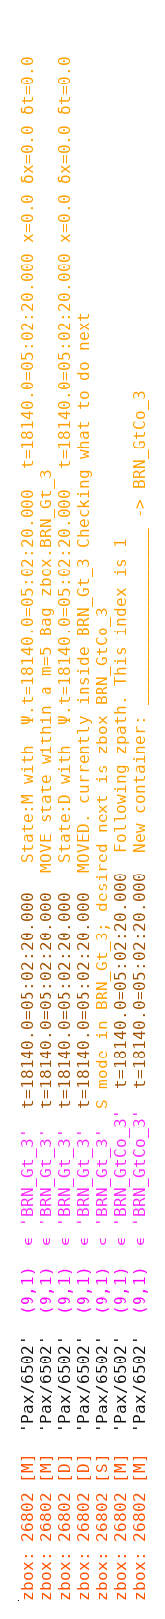
\includegraphics[angle=270,width=16cm]{70_figs/Pax_6502a.eps}\\
\vspace{0.1cm}\\
. . . (many lines)\\
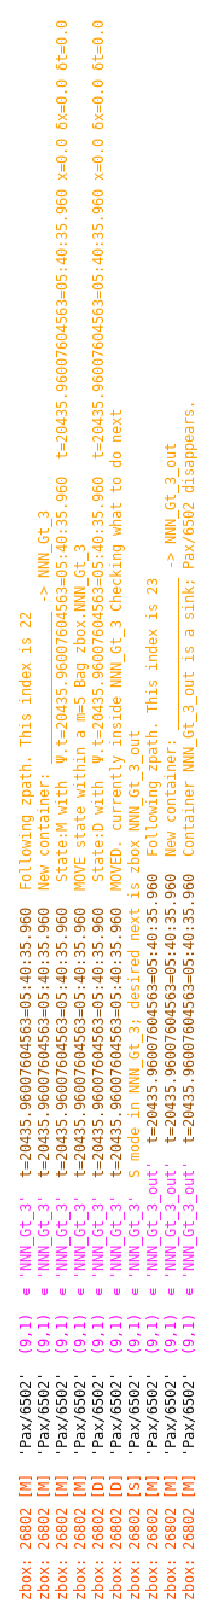
\includegraphics[angle=270,width=16cm]{70_figs/Pax_6502b.eps}\\
\vspace{0.5cm}

It is noted that the Passenger ends his trip by quitting the system at a \emph{Sink} {\tt NNN\_Gt\_3\_out} as expected.
Transitions to a new container always contain the line of several underscores; it is easier to follow the
progress of {\tt Pax/6502} by:\\
\comline{./02\_Run\_simulation.sh v=Pax/6502 | grep \_\_\_\_\_}\\
which appears on the terminal as:\\
\includegraphics[angle=270,width=16cm]{70_figs/Pax_6502.eps}
\vspace{0.5cm}

It is apparent that the passenger travelled from station BRN on {\tt Train\_proto/ML2/1} to station CJC,
then from CJC on {\tt Train\_proto/L10/7} to TTR, and finally on {\tt Train\_proto/L1/12} until
NNN where he quit the system via {\tt NNN\_Gt\_3}.

To follow the trajectory of one of these trains,\\
\comline{./02\_Run\_simulation.sh v=Train\_proto/L10/7 | grep \_\_\_\_\_}\\
which produces the terminal output:\\
\includegraphics[angle=270,width=16cm]{70_figs/Train_L10_7.eps}
\vspace{0.5cm}

The train follows the trajectory expected of a \zobj{zbox} following the
{\tt Train\_L10\_1\_Line} \zobj{zpath}, which from the zsyntax file {\tt \_03\_Paths.zim}
looks like this:
\begin{lstlisting}[mathescape]
# ---- Line L10_1(Hospital Infanta Sofía - Tres Olivos - Puerta del Sur)
[zpath Train_L10_1_Line A=Train n=1 m=Open
 $\Lambda$={ [zs $\phi$=<DEL_Bn_L10_1>]  [zs $\phi$=<Trk_L10_1_DEL_JVJ>]  [zs $\phi$=<JVJ_Bn_L10_1>]
 [zs $\phi$=<Trk_L10_1_JVJ_CVC>]  [zs $\phi$=<CVC_Bn_L10_1>]  [zs $\phi$=<Trk_L10_1_CVC_AEA>]
 [zs $\phi$=<AEA_Bn_L10_1>]  [zs $\phi$=<Trk_L10_1_AEA_CJC>]  [zs $\phi$=<CJC_Bn_L10_1>]
 [zs $\phi$=<Trk_L10_1_CJC_CDC>]  [zs $\phi$=<CDC_Bn_L10_1>]  [zs $\phi$=<Trk_L10_1_CDC_ATÁ>]
 [zs $\phi$=<ATÁ_Bn_L10_1>]  [zs $\phi$=<Trk_L10_1_ATÁ_LAG>]  [zs $\phi$=<LAG_Bn_L10_1>]
 [zs $\phi$=<Trk_L10_1_LAG_PPP>]  [zs $\phi$=<PPP_Bn_L10_1>]  [zs $\phi$=<Trk_L10_1_PPP_PDE>]
 [zs $\phi$=<PDE_Bn_L10_1>]  [zs $\phi$=<Trk_L10_1_PDE_TTR>]  [zs $\phi$=<TTR_Bn_L10_1>]
 [zs $\phi$=<Trk_L10_1_TTR_AMN>]  [zs $\phi$=<AMN_Bn_L10_1>]  [zs $\phi$=<Trk_L10_1_AMN_GMG>]
 [zs $\phi$=<GMG_Bn_L10_1>]  [zs $\phi$=<Trk_L10_1_GMG_NMN>]  [zs $\phi$=<NMN_Bn_L10_1>]
 [zs $\phi$=<Trk_L10_1_NMN_SAA>]  [zs $\phi$=<SAA_Bn_L10_1>]  [zs $\phi$=<Trk_L10_1_SAA_CCU>]
 [zs $\phi$=<CCU_Bn_L10_1>]  [zs $\phi$=<Trk_L10_1_CCU_AIA>]  [zs $\phi$=<AIA_Bn_L10_1>]
 [zs $\phi$=<Trk_L10_1_AIA_CCH>]  [zs $\phi$=<CCH_Bn_L10_1>]  [zs $\phi$=<Trk_L10_1_CCH_BBE>]
 [zs $\phi$=<BBE_Bn_L10_1>]  [zs $\phi$=<Trk_L10_1_BBE_FFU>]  [zs $\phi$=<FFU_Bn_L10_1>]
 [zs $\phi$=<Trk_L10_1_FFU_TOT>]  [zs $\phi$=<TOT_Bn_L10_1>]  [zs $\phi$=<Trk_L10_1_TOT_TEM>]
 [zs $\phi$=<TEM_Bn_L10_1>]  [zs $\phi$=<Trk_L10_1_TEM_LTL>]  [zs $\phi$=<LTL_Bn_L10_1>]
 [zs $\phi$=<Trk_L10_1_LTL_RDL>]  [zs $\phi$=<RDL_Bn_L10_1>]  [zs $\phi$=<Trk_L10_1_RDL_LAA>]
 [zs $\phi$=<LAA_Bn_L10_1>]  [zs $\phi$=<Trk_L10_1_LAA_MAE>]  [zs $\phi$=<MAE_Bn_L10_1>]
 [zs $\phi$=<Trk_L10_1_MAE_MDL>]  [zs $\phi$=<MDL_Bn_L10_1>]  [zs $\phi$=<Trk_L10_1_MDL_MDF>]
 [zs $\phi$=<MDF_Bn_L10_1>]  [zs $\phi$=<Trk_L10_1_MDF_ATL>]  [zs $\phi$=<ATL_Bn_L10_1>]
 [zs $\phi$=<Trk_L10_1_ATL_RCR>]  [zs $\phi$=<RCR_Bn_L10_1>]  [zs $\phi$=<Trk_L10_1_RCR_HIS>]
 [zs $\phi$=<HIS_Bn_L10_1>]  [zs $\phi$=<Sink_L10>]
}]
\end{lstlisting}

Two points are emphasized here. Firstly, in each of the above runs, the full simulation is indeed
being executed; the {\tt -v} option and the {\tt v=...} merely determine
levels of verbosity for either the system as a whole or individual \zobj{zboxen}.
Secondly, the above output is (as mentioned repeatedly) not intended
to be parsed beyond debugging of the system specification.
The \emph{reporting} output, which is indeed intended for this purpose,
is investigated below.

\subsection{Simulation output}
\label{sec:metzimout}

Upon completion (which is most efficiently accomplished without {\tt
  -v}), the file {\tt madrid\_01.zo} will contain the \emph{reporting}
output, every row beginning with {\tt R:}. It is of course much
like the example reporting output exhibited in \Chapref{Chap:SysExm}.

\begin{lstlisting}[mathescape]
R: zbox  i=latlon:40.4123454,-3.70466 ztype=Station,1,1 t=18000.0 R=- state=M
  Z.n=19 label=TDM t0=18000.0 x0=-0.0 t1=18000.0 x1=-0.0 $\delta$t=0.0 l=1 L=0
  Z.n=19 SpaceInside=-55 Z={ TDM_Cc(2,1) TDM_GtCo_1(8,1) TDM_Gt_1(3,1)
    TDM_Gt_1_out(4,1) TDM_GtCo_2(8,1) TDM_Gt_2(3,1) TDM_Gt_2_out(4,1)
    TDM_GtCo_3(8,1) TDM_Gt_3(3,1) TDM_Gt_3_out(4,1) TDM_GtCo_4(8,1)
    TDM_Gt_4(3,1) TDM_Gt_4_out(4,1) TDM_Bn_L1_0(6,1) TDM_Pf_L1_0(5,1)
    TDM_PfCo_L1_0(8,1) TDM_Bn_L1_1(6,1) TDM_Pf_L1_1(5,1) TDM_PfCo_L1_1(8,1)}
R: zbox ztype=Concourse,2,1 t=18000.0 R=- state=M Z.n=0 label=TDM_Cc
  z.label=TDM z.L=0 z.W=1 t0=18000.0 x0=0.0 t1=18000.0 x1=0.0 $\delta$t=0.0 l=1 L=0 z.n=19
R: zbox ztype=Corridor,8,1 t=18000.0 R=- state=M Z.n=0 label=TDM_GtCo_1
  z.label=TDM z.L=0 z.W=1 t0=18000.0 x0=0.0 t1=18000.0 x1=0.0 $\delta$t=0.0 l=1 L=110 z.n=19
R: zbox ztype=Gate,3,1 t=18000.0 R=- state=M Z.n=0 label=TDM_Gt_1 z.label=TDM z.L=0
  z.W=1 t0=18000.0 x0=0.0 t1=18000.0 x1=0.0 $\delta$t=0.0 l=1 L=0 z.n=19

  . . . (many rows)

R: zbox ztype=Train,9,1 t=38338.9315589354 R=- state=M Z.n=32 label=Train_proto/L6/15
  z.label=MLM_Bn_L6_0 z.L=124 z.W=1 t0=38338.9315589354 x0=0.0 t1=38338.9315589354
  x1=0.0 $\delta$t=0.0 l=100 L=1380 Z.n=32 SpaceInside=1348 D="⤷ MLM_Bn_L6_0"
R: zbox ztype=Train,9,1 t=38338.9315589354 R=- state=M Z.n=0 label=Train_proto/L6/57
  z.label=Trk_L6_0_MLM_PPA z.L=749 z.W=1 t0=38338.9315589354 x0=0.0 t1=38341.260456273805
  x1=49.0 $\delta$t=2.328897338403042 l=100 L=1380 Z.n=0 SpaceInside=1380 D=""
R: zbox ztype=Train,9,1 t=38338.9315589354 R=- state=D Z.n=32 label=Train_proto/L6/15
  z.label=MLM_Bn_L6_0 z.L=124 z.W=1 t0=38338.9315589354 x0=0.0 t1=38362.9315589354
  x1=24.0 $\delta$t=24.0 l=100 L=1380 Z.n=32 SpaceInside=1348 D=""  
\end{lstlisting}
with these reporting rows indicating each \zobj{zbox} movement which occured during the
simulation. Since the command-line interface has been used, these are written to a file during
the simulation; if another interface had been used, they would be available for parsing as
they are generated.

The included \emph{TravelTimeTool} tool can used to produce plots and perform comparisons
in terms of passenger travel times. Use of this tool to calibrate the passenger walking
speed in the system is the subject of the following chapter.



